\documentclass[tikz,border=6pt]{standalone}
\usepackage{amsmath}
\begin{document}
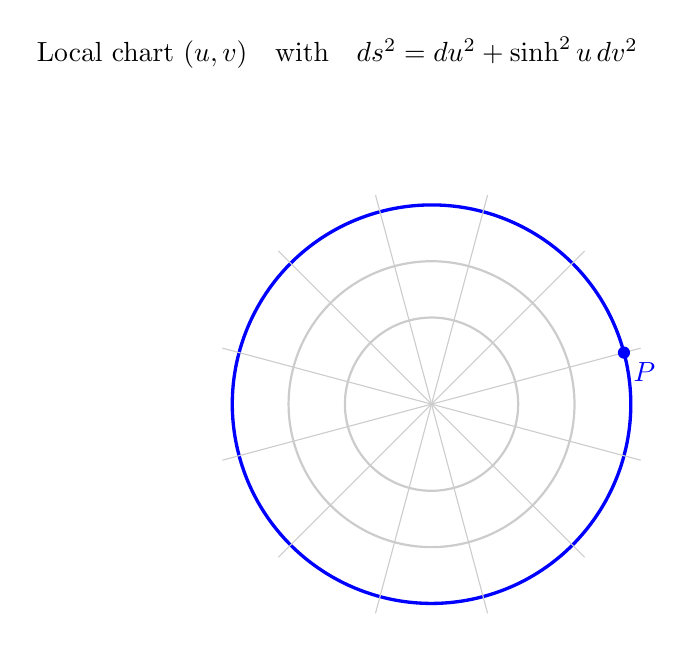
\begin{tikzpicture}[scale=1.1,>=stealth, rotate=15]


% Title & metric
\node[align=center] at (0,4.2)
  {$\text{Local chart }(u,v)\quad\text{with}\quad ds^{2}=du^{2}+\sinh^{2}u\,dv^{2}$};

% Concentric u=const "circles"
\draw[thick,gray!40] (0,0) circle (1.0);
\draw[thick,gray!40] (0,0) circle (1.65);
\draw[very thick,blue] (0,0) circle (2.3); % this is the highlighted u=u_0

% Radial v-lines (equally spaced)
\foreach \ang in {0,30,...,330}{
  \draw[gray!40] (0,0)--({2.5*cos(\ang)},{2.5*sin(\ang)});
}

% Orientation arrow along the highlighted u-curve
%\draw[blue,->,line width=1] ({2.3*cos(20)},{2.3*sin(20)}) arc[start angle=20,end angle=60,radius=2.3];
%\node[blue] at ({2.6*cos(40)},{2.6*sin(40)}) {$v\uparrow$};

% Point P on the highlighted circle
\fill[blue] (2.3,0) circle (2pt) node[below right] {$P$};

% Annotations near P
%\node[align=left,anchor=west] at (2.6,0.3) {$|\partial_u\mathbf r|=1$\\ $|\partial_v\mathbf r|=\sinh u=\tfrac{4}{3}$\\ $\cosh u=\tfrac{5}{3}$};

% Legend for u=const and v=const
%\draw[very thick,blue] (-3.1,3.6)--(-2.6,3.6) node[right,black]{\; $u=\text{const}$};
%\draw[gray!50,thick] (-3.1,3.2)--(-2.6,3.2);
%\draw[gray!50,thick] (-2.85,3.2)--++(0.25,0.43);
%\node[anchor=west] at (-2.6,3.2) {$v=\text{const}$};

\end{tikzpicture}
\end{document}